
\section{Appendix}

\begin{figure}[h!]
\centering
\includegraphics[width=1\textwidth]{checkstyle-checklipse}
\caption{Anwendung von Checkstyle-Standardregeln auf ein Demo-Projekt in Eclipse mithilfe des Plugins ``Checklipse''; zu sehen sind Optimierungsvorschläge auf der Basis der Regeln}
\label{fig:checklipse}
\end{figure}

\newpage

\begin{figure}
\centering
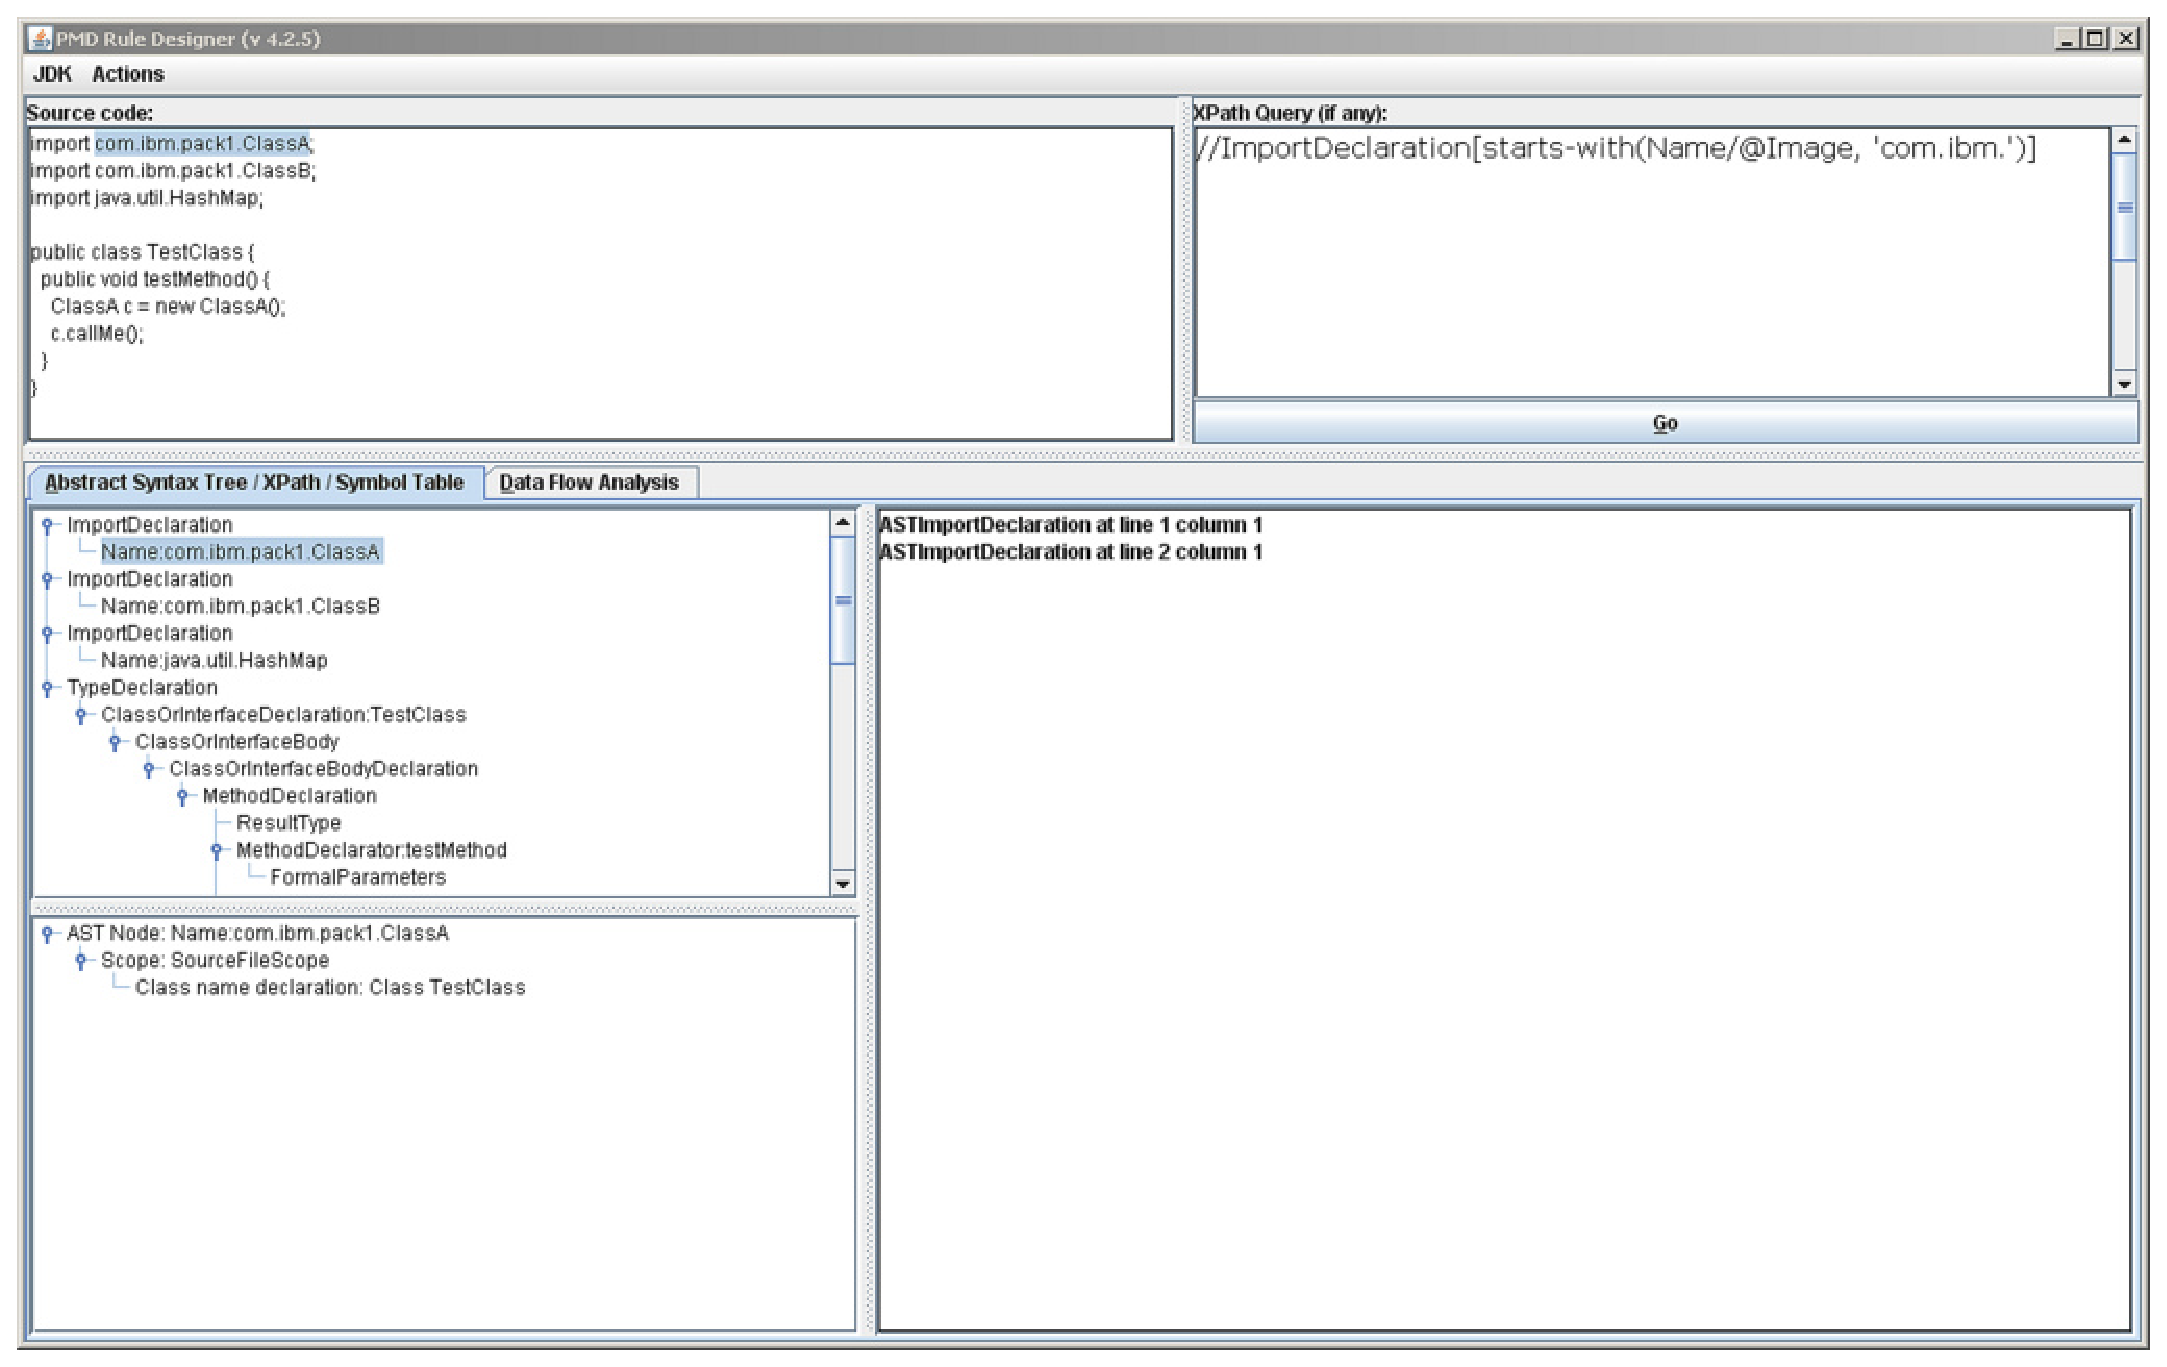
\includegraphics[width=1\textwidth]{pmd-dev}
\caption{Anwendung des Werkzeugs PMD im Rahmen einer statischen Code-Analyse; hier gezeigt ist das Traversieren des AST zum Zwecke des Anlegens eigener Regeln}
\label{fig:pmd}
\end{figure}